\usetikzlibrary{shapes,arrows}

\tikzstyle{input} = [coordinate]
\tikzstyle{output} = [coordinate]
\tikzstyle{block} = [draw, rectangle]
\tikzstyle{sum} = [draw, circle]

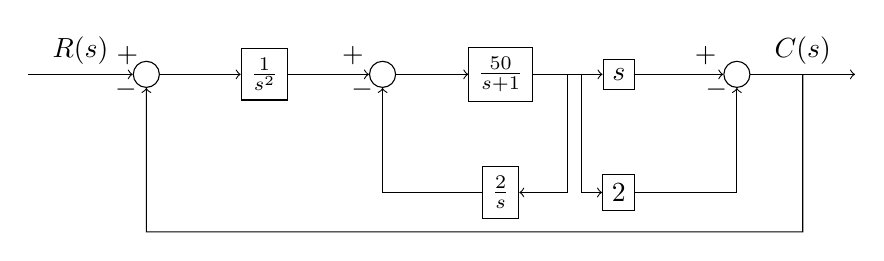
\begin{tikzpicture}[auto,node distance=1.5cm]
	% put the nodes (blocks, sums, etc..) where we want them
	\node [input,name=input] (in) {};
	\node [sum,right of=in] (sum1) {};
	\node [block,right of=sum1] (g1) {$\frac{1}{s^2}$};
	\node [sum,right of=g1] (sum2) {};
	\node [block,right of=sum2] (g2) {$\frac{50}{s+1}$};
	\node [block,right of=g2] (g3) {$s$};
	\node [sum,right of=g3] (sum3) {};
	\node [output,right of=sum3] (out) {};
	\node [block,below of=g3] (h2) {$2$};
	\node [block,below of=g2] (h1) {$\frac{2}{s}$};

	% draw the feedforwards
	\draw [->] (in) -- node {$R(s)$} node[pos=0.95] {$+$} (sum1);
	\draw [->] (sum1) -- (g1);
	\draw [->] (g1) -- node[pos=0.8] {$+$} (sum2);
	\draw [->] (sum2) -- (g2);
	\draw [->] (g2) -- 
		node[name=p2] {}
		node[coordinate,name=p3,right=0.5em] {} 
		(g3);
	\draw [->] (g3) -- node[pos=0.8] {$+$} (sum3);
	\draw [->] (sum3) -- node[name=cs] {$C(s)$} (out);

	% h1 feedback
	\draw [->] (p2) |- (h1);
	\draw [->] (h1) -| node[pos=0.99] {$-$} (sum2);
	
	%h0 feedback
	\node[coordinate,below of=cs,node distance=2.3cm,name=p4] {}; 
	\node[coordinate,below of=sum1,node distance=2cm,name=p5] {};
	\draw [->] (cs) -- (p4) --  (p5) -- node[pos=0.99] {$-$} (sum1);

	%h2 feedforward
	\draw [->] (p3) |- (h2);
	\draw [->] (h2) -| node[pos=0.99] {$-$} (sum3);

\end{tikzpicture}

